\section{Related Work}
%In this section, we briefly review studies about heterogeneous information network and network embedding.

As a newly emerging direction, heterogeneous information network~\citep{shi2017survey} can model complex objects and their rich relations in real scenario. Due to the flexibility of HIN in modeling various kinds of heterogeneous data, many meta-path based search and mining tasks
have been explored in the past couple of years, including clustering~\citep{Sun2012Integrating}, classification~\citep{Ji2011Ranking} and recommendation~\citep{hu2018leveraging}. Considering the plentiful attributes in the nodes, \cite{Li2017Semi} further proposes attributed heterogeneous information network to enrich objects' information content and study the problem of clustering objects in an AHIN. Traditional network mining methods do not pay much attention to node attribute information, which may play important roles in real applications. Therefore, we firstly propose to model the cash-out users detection problem as a classification problem in AHIN.

\begin{figure}[t]
\begin{minipage}[t]{0.45\linewidth}
\centering
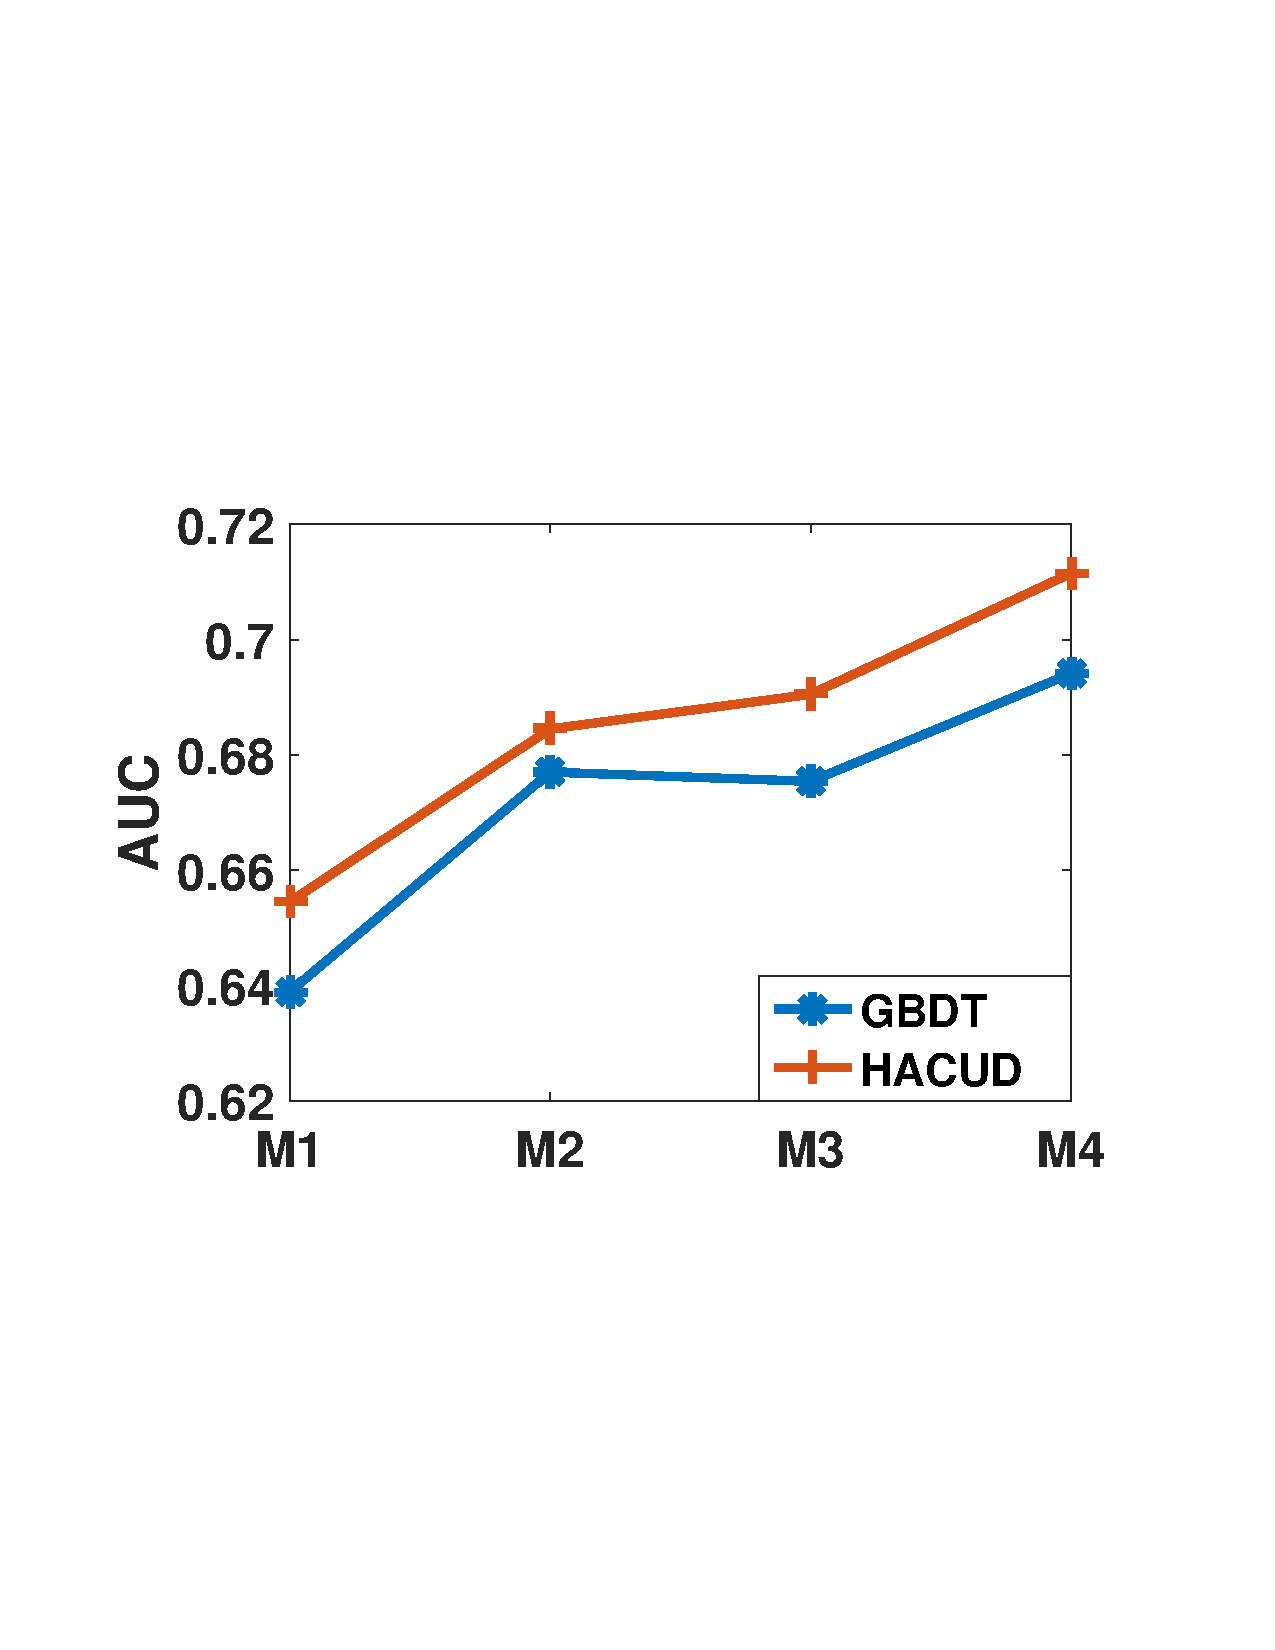
\includegraphics[width=4.1cm]{image/metapath.pdf}
\caption{Impact of different meta-paths on Ten Days Dataset.}
\label{fig-metapath}
\end{minipage}
\begin{minipage}[t]{0.45\linewidth}
\centering
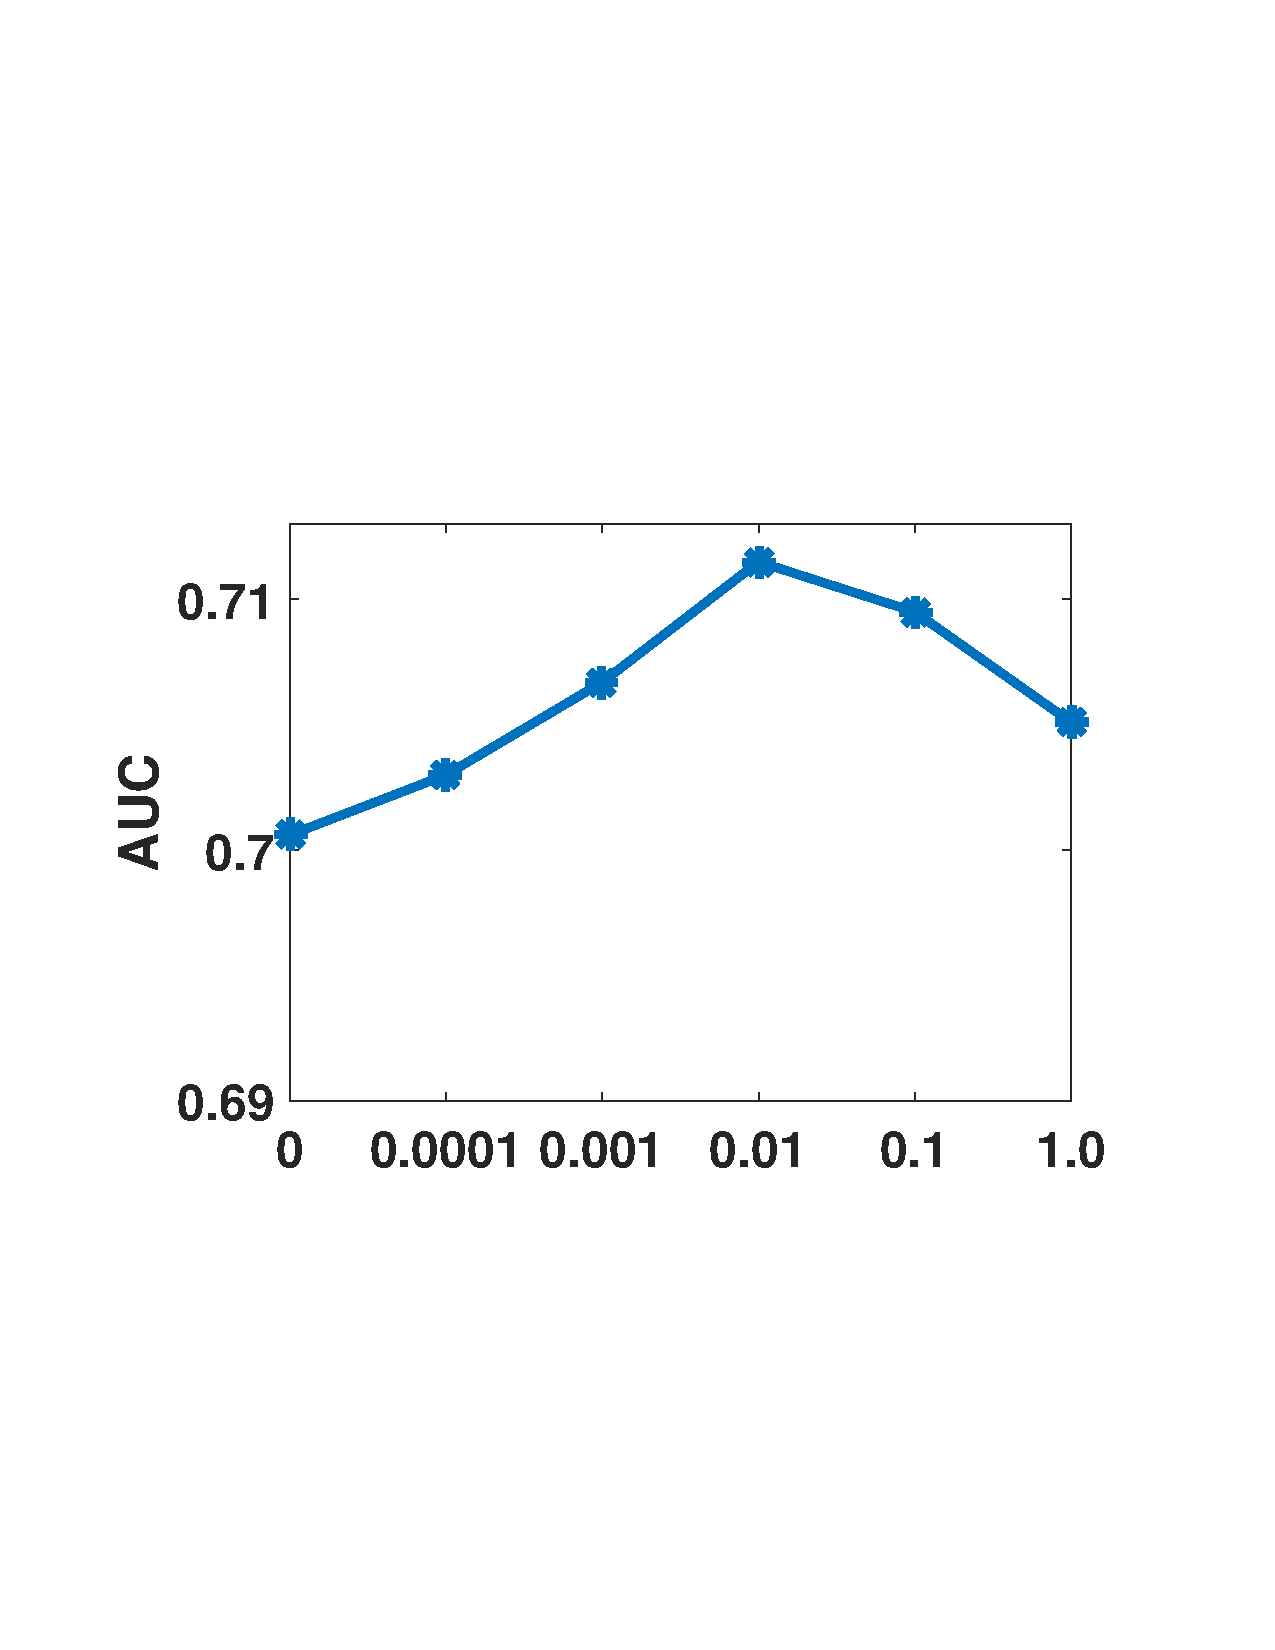
\includegraphics[width=4.1cm]{image/lambda.pdf}
\caption{Impact of parameter $\lambda$  on Ten Days Dataset.}
\label{fig-lambda}
\end{minipage}
\end{figure}

On the other hand, network embedding has shown its potential in structure feature extraction and has been successfully applied in many data mining tasks. Early network embedding methods focus on homogeneous network, which usually utilize network context information to represent nodes, \eg random walk based context~\citep{Perozzi2014DeepWalk,grover2016node2vec}, network neighborhood~\citep{wang2016structural,Tang2015LINE}, high order network proximity~\citep{Cao2015GraRep}. Recently, attention is increasingly shifting towards heterogeneous network.  \cite{dong2017metapath2vec} obtain the context of nodes with meta-path based random walk and learn the HIN embedding through heterogeneous skip-gram model, while \cite{Fu2017HIN2Vec} capture rich relation semantics via neural network. Moreover, there are also several works attempting to fully analyze networks via embedding methods with features and labeled data, including GCN~\citep{Kipf2016Semi}, Structure2vec~\citep{dai2016discriminative} and so on. Unfortunately, these methods are usually designed for specific task and only exploit partial information in networks, therefore they cannot be directly applied in the AHIN and the cash-out user detection problem for promising performance.